two types of evaluation: usability and ??


\section{Usability Study}

%\subsection{Set-up}
%\label{evaluation-setup}

\begin{figure}[!b]
	\centering
	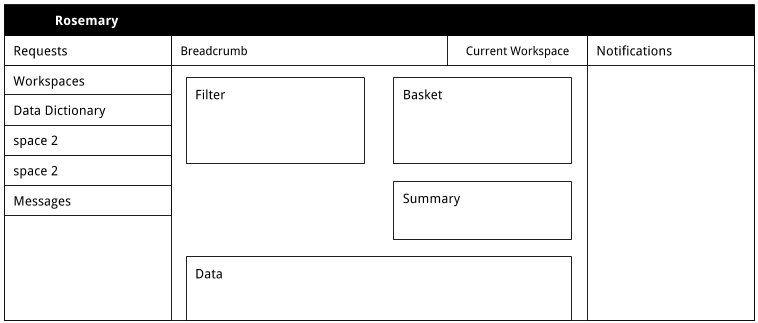
\includegraphics[width=1.0\linewidth]{images/evaluation-layout}
	\caption{
		Wireframe of the Rosemary layout, showing the data management features: filter, view, select. \silvia{this fig can go to chap 3, under UI design (which is missing ;-). put here a screenshot instead (as proof that the system works). Add arrows and notes to the screenshot to show the things that you need to refer to in the text for the evaluation (maybe boxes as in the wire-frame??}
	}
	\label{fig:evaluation-layout}
\end{figure}

All evaluations were done in an informal open-talk setting with no predefined questions.
First, the purpose of the meeting was explained in a few sentences.
Each user had to perform tasks using the prototype according to the assigned case: researcher, committee, administrator.
There were three testers, and some were assigned two cases because they fit in the field of experience of the respective user role.

Tasks were described according to the system usage schema presented in figure \ref{fig:brainstorm-after}).
The interviewer only gave directions during the evaluation after the tester indicated that they did not know how to proceed.
If the tester struggled with a task the interviewer tried to encourage the tester to think aloud.
From this the process, bottlenecks and design flaws of the system were identified.
Also, testers were asked to provide design or process alternatives. \silvia{not clear what "process" means here. did they have new ideas about system functions? or presentation? or the sequence? be explicit}

\silvia{explain how you prepared the prototype (where deployed?), with fake data, preconfigured user accounts and roles, etc}

\begin{figure}[th]
	\centering
	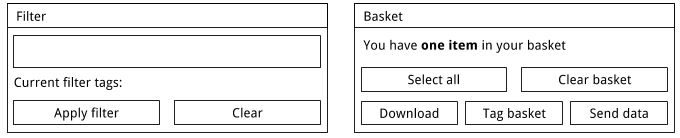
\includegraphics[width=1.0\linewidth]{images/evaluation-basket-layout}
	\caption{
		Wireframes of the Rosemary filter and basket layout, showing the search and select data management tools.
		These wireframes are the more detailed versions of the filter and basket blocks shown in figure \ref{fig:evaluation-layout}.
	}
	\label{fig:evaluation-basket-layout}
\end{figure}

%\subsection{Cases}
%\label{evaluation-cases}

The  cases presented below are loose transcripts of the evaluation sessions.
Refer to figure \ref{fig:evaluation-layout} for clarification on the used terms.
Identified problems and possible improvements are summarised in the  section \ref{}.

\paragraph{Researcher Role.}
From all the cases this is arguably the largest as it has the most extensive (implemented) functions.
Therefore, all the testers performed the researcher tasks to find more flaws or give more support to flaws found with both testers.
The tasks that had to be performed were: search the data dictionary for headers, use these data headers to compose a Request, download the requested data. \silvia{no submit request?}

%Finding the data dictionary was not a big problem for the testers, however it was unclear that the dictionary itself was (like all data views) a workspace.
%Having a separate workspace for each of the requests made sense but the dictionary should be a entity that exists on itself.

Finding the data dictionary was not a big problem for the testers.
The next step is filtering, which is relatively easy as the input (see left side of figure \ref{fig:evaluation-basket-layout}) is text based and the search itself is fuzzy.
Dictionary items can be sought for based on name, description, and keywords.
Because in the prototype the descriptions are nonsense, it was difficult to find the wanted data headers.
Two of the testers did not notice that the search is instantaneous (like google search).
This resulted in pressing enter and clicking the `apply filter' button multiple times before noticing that the data had already changed at the bottom of the screen.
One of the testers prefers to search the data analogically (\ie{} print the data) and later select the wanted items in the interface.

The filter function plus the nonsense data made it rather hard for the testers to find the desired headers, they were asked to select a couple of random headers to start a request with.
Selection was straight-forward but the testers did not notice that selected items were added to the `basket' (see right side of figure \ref{fig:evaluation-basket-layout}).
Therefore, two asked `how do I keep this selection when I start searching again?'.
This also resulted in two of the testers using the `select all' function on the basket. 
Clicking this will make a selection of \emph{all} the items in the workspace, basically overwriting the previous basket and losing all the progress.

To proceed in the task of making a request the testers looked for a button on the basket.
However, the buttons (see right side of figure \ref{fig:evaluation-basket-layout}) are specific to a raw data view and do not make sense in a dictionary view of the system.
The testers needed to be explained that the basket is kept in the back of the system and can be used over multiple views.
Clicking the request button at the top left of the screen is the correct action, then selecting `new request' results in a form with the basket attached to the end showing which items were selected.

Data download is straight-forward, this is done by going to the correct workspace from the menu on the left, selecting the wanted items (or select all), and clicking the `download' button.
No problems were found here, however one of the testers noted that in principle \emph{all} data will be downloaded every time.

\paragraph{Committee Member Role.}
The committee tasks are the shortest as the list contains one function: request approval. \silvia{a bit poor. maybe also find which approvals are needed, which have been already done?}
Viewing requests that are ready for approval is done by selecting the `request' button from the left menu.
Now a list is shown of all these requests and the data that is necessary for making the decision.
Approval is given (or not) by selecting a approve or disprove button, a vote remains open for change until all committee members have casted their vote.
What vote was cast is shown both with a symbol (V/X) as with a colour (green/red) which was directly clear to the tester.

Communication functions are built into the view.  
\silvia{not clear: clicking a request,  redirects to a `new message' view which already has all affected committee members in the `to' field.}
There was a suggestion to add a comments thread to the request itself, instead of the separate message construction.
Furthermore, the redirect was confusing for the tester as the expectation was that it would lead to more information on the request.
\silvia{so which information about the request was presented?}

\paragraph{Data administrator Role.}
Lastly, the data administrator performed the user management functions.
The user overview is not complex in functionality, a list of users is shown.
Each with buttons to perform the following actions: make committee member, make active, approve.
This was clear and would be easy to use in a real-life scenario.
However, the tester noted that there are some process flaws.
If one of the users of the system changes institutions most of the time the data manager is not informed, this is left to the P.I.s.
Therefore the system should contain support functions for non-administrators to view the list of users and communicating with the data manager about what actions should be taken.